
\chapter{Methodology}

\section{Research context}

Swarmia is a Software as a Service tool for software development teams. Teams utilize Swarmia to measure their performance and find potential places of improvement in their development pipeline. Swarmia is designed to help teams work in a self-managed manner.

To provide insight to the client teams, Swarmia integrates with issue trackers like Jira and version control systems like GitHub. The teams are then provided with insights accessible to all team members through the Swarmia web application. In addition, Swarmia can be configured to push updates to the team's Slack channel. A team of any size can use Swarmia: the teams include both working within software companies and in-house development teams of non-software companies. 

One of the features in Swarmia is called Working Agreements. Teams can configure up to eight agreements, generally described as team norms or collaboration guidelines. The agreements are selected from a predefined list of options: each team can customize them to suit their use case. For example, a team could agree that they want to enforce linking pull requests to issues. Swarmia would then track the set condition automatically and inform the teams about the status of the agreement. 

Working agreement options in Swarmia are presented in Figure \ref{fig:WorkingAgreements}.

\begin{table}[h!]
\centering
\begin{tabular}{ |c|c| } 
\hline
option in Swarmia & computer readable \\ [0.5ex] 
\hline\hline
Avoid pushing directly to the default branch & no\_direct\_pushes\_to\_main\_branch \\
Avoid working alone & min\_issue\_contributors  \\
Limit issues in progress & wip\_issues  \\
Limit pull requests in progress & wip\_pull\_requests \\
Link pull requests to issues & pull\_request\_linking  \\
Reduce issue cycle time & max\_issue\_age  \\
Reduce pull request cycle time & max\_pull\_request\_age \\
Reduce pull request review time & max\_pull\_request\_review\_time  \\
\hline
\end{tabular}
\caption{Working Agreement options}
\label{tab:workingAgreements}
\end{table}

\begin{figure}[h]
    \begin{center}
        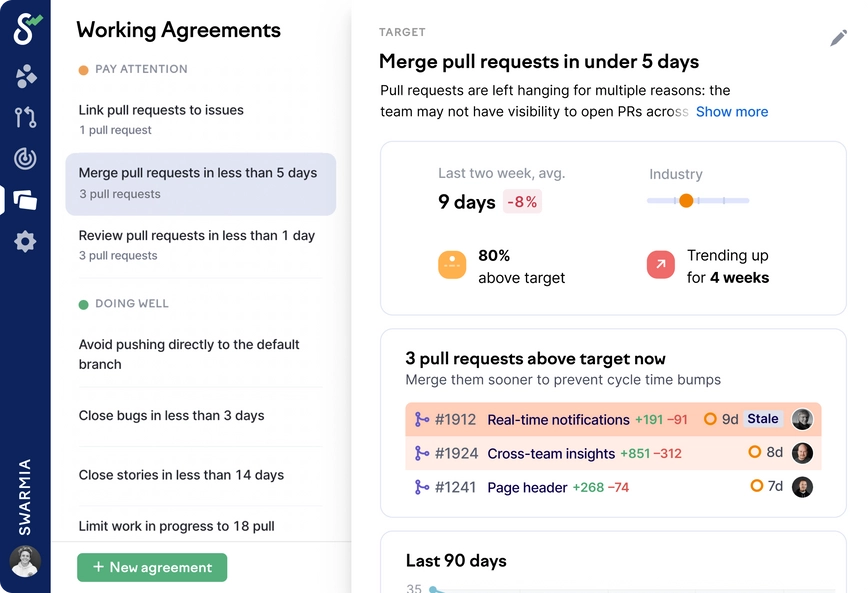
\includegraphics[width=13.5cm]{LaTeX/images/improvement.png}
        \caption{Working Agreements in Swarmia}
        \label{fig:WorkingAgreements}
    \end{center}
\end{figure}

\section{Data}

The data collected by Swarmia includes, but is not limited to, pull requests, issues, and failed deployments. Furthermore, Swarmia has read-only access to the source code, which is used to estimate the complexity of the change in question. Swarmia never stores client code but instead calculates the size of the change bundle and stores it in a separate database. 

Processing of the data is done in Google's BigQuery data warehouse service. Most of the information needed is already collected at Swarmia for business intelligence purposes but needs to be structured in a suitable format. The data flow is shown in Figure \ref{fig:dataFlow}.

\begin{figure}[ht]
\centering
\begin{tikzpicture}[
    every node/.style={align=center, minimum height=1em, minimum width=1cm,node distance=0.7cm},
]

%Nodes
\node[entity]      (teamswa)        {active teams with WA adoption};
\node[entity]      (teams)          [above=of teamswa] {team basic info};
\node[entity]      (snapshots)       [left=of teams] {team snapshots};
\node[entity]       (mau)           [right=of teams] {MAU};
\node[entity]      (ctwa)       [below=of teamswa] {cycle times with WA adoption};
\node[entity]      (cycletimes)       [left=of ctwa]     {cycle times};
\node[entity]      (adoption)       [left=of snapshots] {WA adoption};
\node[entity, fill=gray!20]       (lm)        [below=of ctwa] {linear model input data};

%Lines
\draw[->] (cycletimes.east) -- (ctwa.west);
\draw[->] (ctwa.south) -- (lm.north);
\draw[->] (teamswa.south) -- (ctwa.north);
\draw[->] (teams.south) -- (teamswa.north);
\draw[->] (snapshots.south) -- (teamswa.north);
\draw[->] (mau.south) -- (teamswa.north);
\draw[->] (adoption.south) -- (teamswa.north);

\end{tikzpicture}
\caption{Data flow in BigQuery}
\label{fig:dataFlow}
\end{figure}


\newcommand*\rot{\rotatebox{90}}
\begin{table}[ht]
\begin{center}
\begin{tabular}{|c|c|c|c|c|c|c|c|c|c|c|c|c|c|} 
\hline

No & A & B & C & D & E & F & G & H & ct\_days & slack\_users & daily\_digest \\ [0.5ex]
\hline\hline

1 & 0 & 1 & 0 & 0 & 0 & 0 & 1 & 0 & 1.3 & 2 & 0 \\
2 & 0 & 1 & 0 & 0 & 0 & 0 & 0 & 1 & 0.00031 & 0 & 0 \\ 
3 & 1 & 0 & 1 & 0 & 0 & 0 & 1 & 0 & -0.46 & 4 & 1 \\
4 & 0 & 0 & 0 & 0 & 0 & 0 & 0 & 1 & -0.058 & 5 & 1 \\
5 & 0 & 1 & 1 & 0 & 1 & 1 & 1 & 1 & -1.8 & null & 1 \\

\hline
\end{tabular}
\caption{Sample rows of lm\_data}
\label{tab:dataExample}
\end{center}
\end{table}


For this study, weekly aggregates of team metrics were exported from the Swarmia backend to BigQuery. This data set is called "team pr cycle times" in Figure \ref{fig:dataFlow}. These metrics were joined with basic team information, working agreement usage, and team member activity. Finally, team identifiers and timestamps were removed so the data points would be independent. A resulting data sample is displayed in Table \ref{tab:dataExample}.

\section{Research questions}

The main research question of this thesis is to look into how teams use Working Agreements: which share of Swarmia teams use the feature and how these teams have configured their Working Agreements setup. 

The second research question is to determine if Working Agreements can enhance productivity in software development teams. The hypothesis based on previous research is that as Working Agreements promote methods that accelerate software development, they should directly impact the team's productivity. We will look into the Working Agreement composition in different teams and find out which agreements impact the teams' performance most. 

\section{Approach}

To answer RQ1, data from Swarmia is used to determine how many of the teams have enabled which Working Agreements. Furthermore, we look into how many Working Agreements teams usually have in use and what parameters they have configured in Swarmia: for example, what is their WIP limit in \textit{Limit issues in progress} agreement? Lastly, team characteristics such as team size and their connection to the Working Agreements setup are analyzed. The RQ1 is approached with simple SQL queries. 

To answer RQ2, data from all teams using the Working Agreements feature is collected and analyzed. Historical activity data is pulled from the teams' source control repositories. The data is aggregated weekly for 24 months: some teams have been clients for longer than two years, and some for a shorter amount. This should be fine, as averages are used, and the data collection period is not a variable in the analysis.

The key metric used in the analysis is the Pull Request Cycle Time (PRCT). Even though Swarmia exports data from issue trackers, these data sources were left out of the analysis based on the scope of the thesis. The analysis is done in BigQuery in line with Swarmia's privacy policy. In addition to a standard SQL query engine, BigQuery offers machine learning capabilities. For this thesis, the inbuilt linear regression feature was utilized. Figure \ref{fig:dataFlow} presents the data flow before building the regression model. 

In linear regression, we look at the relationship between the independent and dependent variables. The dependent variable is the one that, as a hypothesis, depends on the values of the independent variables. Respectively, the independent variables are the configuration of working agreements, team member metrics, and Slack notification settings. 

\definecolor{cor-very-weak}{HTML}{BBBBBB}
\definecolor{cor-weak}{HTML}{EEBD84}
\definecolor{cor-moderate}{HTML}{F47461}
\definecolor{cor-strong}{HTML}{F47461}
\definecolor{cor-very-strong}{HTML}{8B0000}

\begin{table}[ht]
\centering
\resizebox{\columnwidth}{!}{
\begin{tabular}{c c c c c c c c c c c c c}

& A & B & C & D & E & F & G & H & ga & sw & sl & dd\\ \hline
A & \textcolor{cor-very-strong}{1.0} & \textcolor{cor-moderate}{0.49} & \textcolor{cor-weak}{0.28} & \textcolor{cor-very-weak}{0.16} & \textcolor{cor-weak}{0.29} & \textcolor{cor-very-weak}{0.15} & \textcolor{cor-moderate}{0.42} & \textcolor{cor-weak}{0.24} & \textcolor{cor-very-weak}{-0.09} & \textcolor{cor-very-weak}{-0.04} & \textcolor{cor-very-weak}{-0.03} & \textcolor{cor-weak}{0.2}\\ \hline
B &  & \textcolor{cor-very-strong}{1.0} & \textcolor{cor-weak}{0.23} & \textcolor{cor-very-weak}{0.18} & \textcolor{cor-weak}{0.32} & \textcolor{cor-weak}{0.31} & \textcolor{cor-strong}{0.64} & \textcolor{cor-weak}{0.39} & \textcolor{cor-very-weak}{-0.07} & \textcolor{cor-very-weak}{0.02} & \textcolor{cor-very-weak}{0.06} & \textcolor{cor-weak}{0.23}\\ \hline
C &  &  & \textcolor{cor-very-strong}{1.0} & \textcolor{cor-weak}{0.25} & \textcolor{cor-weak}{0.26} & \textcolor{cor-very-weak}{0.16} & \textcolor{cor-weak}{0.24} & \textcolor{cor-weak}{0.35} & \textcolor{cor-very-weak}{-0.1} & \textcolor{cor-very-weak}{0.0} & \textcolor{cor-very-weak}{-0.06} & \textcolor{cor-very-weak}{0.09}\\ \hline
D &  &  &  & \textcolor{cor-very-strong}{1.0} & \textcolor{cor-weak}{0.3} & \textcolor{cor-weak}{0.25} & \textcolor{cor-very-weak}{0.15} & \textcolor{cor-weak}{0.3} & \textcolor{cor-very-weak}{0.03} & \textcolor{cor-very-weak}{0.09} & \textcolor{cor-very-weak}{0.0} & \textcolor{cor-very-weak}{0.03}\\ \hline
E &  &  &  &  & \textcolor{cor-very-strong}{1.0} & \textcolor{cor-moderate}{0.58} & \textcolor{cor-weak}{0.28} & \textcolor{cor-moderate}{0.43} & \textcolor{cor-very-weak}{-0.09} & \textcolor{cor-very-weak}{0.01} & \textcolor{cor-very-weak}{-0.02} & \textcolor{cor-very-weak}{0.15}\\ \hline
F &  &  &  &  &  & \textcolor{cor-very-strong}{1.0} & \textcolor{cor-weak}{0.32} & \textcolor{cor-weak}{0.34} & \textcolor{cor-very-weak}{-0.03} & \textcolor{cor-very-weak}{0.08} & \textcolor{cor-very-weak}{0.05} & \textcolor{cor-very-weak}{0.19}\\ \hline
G &  &  &  &  &  &  & \textcolor{cor-very-strong}{1.0} & \textcolor{cor-weak}{0.3} & \textcolor{cor-very-weak}{-0.01} & \textcolor{cor-very-weak}{0.03} & \textcolor{cor-very-weak}{0.08} & \textcolor{cor-weak}{0.32}\\ \hline
H &  &  &  &  &  &  &  & \textcolor{cor-very-strong}{1.0} & \textcolor{cor-very-weak}{-0.09} & \textcolor{cor-very-weak}{0.0} & \textcolor{cor-very-weak}{-0.01} & \textcolor{cor-very-weak}{0.1}\\ \hline
ga &  &  &  &  &  &  &  &  & \textcolor{cor-very-strong}{1.0} & \textcolor{cor-strong}{0.79} & \textcolor{cor-strong}{0.78} & \textcolor{cor-very-weak}{-0.18}\\ \hline
sw &  &  &  &  &  &  &  &  &  & \textcolor{cor-very-strong}{1.0} & \textcolor{cor-very-strong}{0.84} & \textcolor{cor-very-weak}{-0.07}\\ \hline
sl &  &  &  &  &  &  &  &  &  &  & \textcolor{cor-very-strong}{1.0} & \textcolor{cor-very-weak}{-0.01}\\ \hline
dd &  &  &  &  &  &  &  &  &  &  &  & \textcolor{cor-very-strong}{1.0}\\ \hline

\end{tabular}
}

\caption{Correlation matrix. The stronger the correlation, the darker the color. ga=github\_authors, sw=swarmia\_users, sl=slack\_users, dd=daily\_digest}
\label{tab:correlationMatrix}
\end{table}

Pearson correlation coefficient for independent variables is calculated in Table \ref{tab:correlationMatrix} to ensure the data is compatible with linear regression analysis: two variables should not correlate for the model to work as expected. The most considerable correlation encountered is the of slack\_users and swarmia\_users with a value of 0.84. The pairs with high correlation deal with the same themes, for example, WAs related to pull requests. Even though some of the WAs correlate, the data can be used for the model with slight modifications: github\_authors and swarmia\_users were dropped to include only the team member metric, slack\_users. 

Linear regression can be formulated as follows:

\begin{equation}
Y = \beta_0 + \beta_i X_i + \beta_{i+1} X_{i+1} + \ldots + \beta_n X_n + \epsilon
\end{equation}


where
\begin{description}
\item[$Y$] is dependent variable
\item[$\beta_0$] is constant coefficient (intercept)
\item[$\beta_i$] is slope for $X_i$
\item[$X_i$] is independent variable
\item[$\epsilon$] is error
\end{description}

The training data is passed to linear regression in a form presented in Table \ref{tab:trainingDataStructure}. The data has gone through two significant modifications to suit linear regression. First, we calculated an average PRCT for each team before they enabled any working agreements. This average is then subtracted from each row PRCT to achieve a normalized data set: the aim is to diminish the differences between teams to achieve comparable PRCTs. Secondly, WA activation dates are mapped to Boolean values for each row: the value is zero if WA has not been activated yet and one if it has.

\begin{table}
\begin{center}
\begin{tabularx}{\textwidth}{ |l|X| } 
\hline
parameter & description \\ [0.5ex] 
\hline\hline
wip\_pull\_requests & WA status \\
max\_pull\_request\_age & WA status \\
no\_direct\_pushes\_to\_main\_branch & WA status \\
min\_issue\_contributors  & WA status \\
wip\_issues & WA status \\
max\_issue\_age  & WA status \\
max\_pull\_request\_review\_time  & WA status \\
pull\_request\_linking  & WA status \\
ct\_days  & normalized cycle time in days \\
github\_authors & Pull request authors \\
swarmia\_users & MAU in Swarmia team \\
slack\_users & Swarmia users with Slack notifications \\
daily\_digest & team's Slack daily digest status \\
\hline
\end{tabularx}
\caption{Linear regression training data structure}
\label{tab:trainingDataStructure}
\end{center}
\end{table}




At first, there were three team member-related metrics: github\_authors, swarmia\_users, and slack\_users. Swarmia\_users did not have statistical significance and correlated pretty strongly with github\_users. In the end, out of the three metrics, only slack\_users was retained for the final model.

The model was also run with PRCT components: time in progress, in review, and ready to merge. The aim was to investigate which part of the process the independent variables mainly influenced. Only modeling against in-progress cycle time (IPCT) produced results with statistical significance.  
